\documentclass[../../main.tex]{subfiles}
\begin{document}

\begin{flushright}
\footnotesize\textit{【自動文字起こし・要確認】}
\end{flushright}

{\bf [解]}
$f(x)=x\sin x\ (x\ge0)$，$f'(x)=\sin x+x\cos x$である．$f'(\pi/2)=1$だから，$x=\pi/2$での法線は$y=-x+\pi$である．

\begin{figure}[htb]
\centering
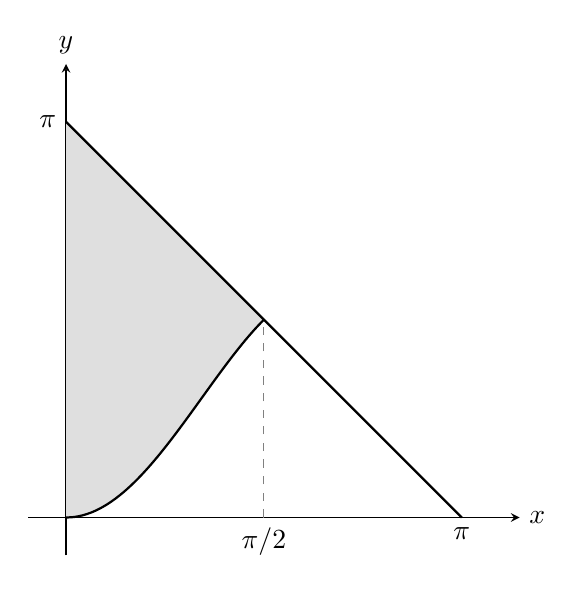
\begin{tikzpicture}[scale=1.6, >=stealth]
  \draw[->] (-0.3,0) -- (3.6,0) node[right] {$x$};
  \draw[->] (0,-0.3) -- (0,3.6) node[above] {$y$};
  \fill[gray!25] plot[domain=0:1.5708, smooth] (\x,{\x*sin(\x r)}) -- (0,3.1416) -- cycle;
  \draw[domain=0:1.5708, smooth, thick] plot (\x,{\x*sin(\x r)});
  \draw[thick] (0,3.1416) -- (3.1416,0);
  \draw[gray, dashed] (1.5708,0) -- (1.5708,1.5708);
  \node[below] at (1.5708,0) {$\pi/2$};
  \node[below] at (3.1416,0) {$\pi$};
  \node[left] at (0,3.1416) {$\pi$};
\end{tikzpicture}
\caption{$y=f(x)$，法線，$y$軸で囲まれる図形（斜線部）}
\end{figure}

これを$x$軸まわりに回転してできる立体の体積は
\begin{align*}
V=\pi\int_0^{\pi/2}\left[(-x+\pi)^2-x^2\sin^2x\right]dx\quad\cdots①
\end{align*}

ここで，
\begin{align*}
\int_0^{\pi/2}x^2\sin^2x\,dx=\int_0^{\pi/2}\frac12x^2(1-\cos2x)\,dx\quad\cdots②
\end{align*}
であり，
\begin{align*}
\int_0^{\pi/2}x^2\cos2x\,dx=\left[\frac{x^2}2\sin2x+\frac{2x}4\cos2x-\frac28\sin2x\right]_0^{\pi/2}=-\frac\pi4
\end{align*}

から，②に代入して
\begin{align*}
\int_0^{\pi/2}x^2\sin^2x\,dx=\frac12\left[\frac13x^3\right]_0^{\pi/2}+\frac\pi8=\frac1{48}\pi^3+\frac18\pi\quad\cdots③
\end{align*}

又，
\begin{align*}
\int_0^{\pi/2}(x-\pi)^2\,dx=\left[\frac13x^3-\pi x^2+\pi^2x\right]_0^{\pi/2}=\frac7{24}\pi^3\quad\cdots④
\end{align*}

③④を①に代入して
\begin{align*}
V&=\pi\left\{\frac7{24}\pi^3-\frac1{48}\pi^3-\frac18\pi\right\}\\
&=\pi\left(\frac{13}{48}\pi^3-\frac18\pi\right)．
\end{align*}

\newpage

\end{document}
